% ============================================================================
% Title: Stochastic Thermodynamics of Single-Cell Commitment:
%        A Non-Equilibrium Analysis of Bacillus subtilis Sporulation
% Author: Eugênio Simão
% Status: working draft (July 2026)
% Target: Physical Review X / eLife (physics) / PRE
%
% This version frames the work explicitly around NESM + SHPN.
% Biology (Fujita constraints) is the validation prerequisite, not the
% main result. The main result is the thermodynamic characterisation of
% single-cell commitment as an open non-equilibrium system.
%
% Structure plan: workspace/projects/thesis/manuscript/parts/NESM_manuscript_plan.tex
% ============================================================================

\documentclass[11pt,a4paper]{article}

\usepackage[utf8]{inputenc}
\usepackage[T1]{fontenc}
\usepackage[english]{babel}
\usepackage{amsmath,amssymb,amsthm}
\usepackage{booktabs}
\usepackage{geometry}
\usepackage{graphicx}
\usepackage{hyperref}
\usepackage{cleveref}
\usepackage{microtype}
\usepackage[table]{xcolor}
\usepackage{colortbl}
\usepackage[font=small,labelfont=bf]{caption}
\usepackage{setspace}
\usepackage[right]{lineno}

\geometry{margin=2.5cm}
\hypersetup{colorlinks=true,linkcolor=blue!50!black,
            citecolor=blue!50!black,urlcolor=blue!50!black}

\crefname{figure}{Fig}{Figs}
\Crefname{figure}{Fig}{Figs}

% ── Math macros ──────────────────────────────────────────────────────────────
\newcommand{\kB}{k_{\mathrm{B}}}
\newcommand{\Gs}{G_s}
\newcommand{\Ge}{G_E}
\newcommand{\thetaeff}{\theta_{\mathrm{eff}}}
\newcommand{\DeltaF}{\Delta F}
\newcommand{\CV}{\mathrm{CV}}
% EPR (entropy production rate)
\newcommand{\EPR}{\dot{\sigma}}
% Trajectory EPR
\newcommand{\TrajEPR}[1]{\sigma[#1]}
% Thermodynamic force / affinity
\newcommand{\aff}{\mathcal{A}}
% Topological load
\newcommand{\etaL}{\eta_{\mathrm{L}}}
% Critical exponent
\newcommand{\gsub}{\gamma_{\mathrm{sub}}}
% Critical nutrient
\newcommand{\Nc}{N_{\mathrm{c}}}
% Time-reversed trajectory
\newcommand{\trev}[1]{\tilde{#1}}

% ─────────────────────────────────────────────────────────────────────────────
\begin{document}
\doublespacing
\linenumbers
\vspace*{0.2in}

% ── Title and author ─────────────────────────────────────────────────────────
\begin{flushleft}
{\Large
\textbf{Stochastic Thermodynamics of Single-Cell Commitment:
A Non-Equilibrium Analysis of \textit{Bacillus subtilis} Sporulation}
}
\newline
\\
Eug\^{e}nio Sim\~{a}o$^{1,*}$
\\
\bigskip
\textbf{1} Department of Computer Science, Universidade Federal de Santa
Catarina (UFSC), Ararangu\'a, Santa Catarina, 88906-072, Brazil
\\
\bigskip
* eugenio.simao@ufsc.br
\end{flushleft}

% ─────────────────────────────────────────────────────────────────────────────
\section*{Abstract}
% ─────────────────────────────────────────────────────────────────────────────

Cells commit irreversibly to differentiation programmes — sporulation,
apoptosis, cell-cycle entry — yet the thermodynamic cost and universality
class of such decisions have never been characterised at the single-cell
level.
Classical thermodynamics is inapplicable to small, far-from-equilibrium
biological systems; stochastic thermodynamics (Seifert 2012), which
provides exact trajectory-level entropy production for Markov chains of
any size, offers a principled alternative.
Here we introduce the Signal Hierarchical Petri Net (SHPN) formalism as the
computational substrate for single-cell non-equilibrium statistical
mechanics (NESM): its arc semantics map directly onto the thermodynamic
ports of an open driven system, and five measurable thermodynamic
quantities --- topological load $\etaL$, dimensionless work $W/\kB T$,
critical nutrient level $\Nc$, sub-critical exponent $\gsub$, and
per-transition entropy production rate (EPR) decomposition --- are
derivable from the network topology and stochastic dynamics alone.
Applied to \textit{Bacillus subtilis} sporulation, the framework
reproduces three independent experimental constraints from Fujita \&
Losick (2005) and reveals that the commitment transition is
non-mean-field ($\gsub = 0.150 \pm 0.044$, 19$\sigma$ below $\gsub^{\mathrm{MF}}
= 0.5$), the critical threshold lies at $\Nc = 1346\,\mu$M, and 97.5\%
of the stochastic EPR is concentrated at the sensing step (KinA
autophosphorylation), not the execution programme.
These results establish SHPN as a natural language for stochastic
thermodynamics of regulatory decision circuits and provide a framework
applicable to any commitment network with known topology.
\vspace{0.5em}
\noindent\textit{Keywords:} stochastic thermodynamics, non-equilibrium
statistical mechanics, Petri nets, sporulation, critical phenomena,
entropy production, single-cell biophysics.

% ─────────────────────────────────────────────────────────────────────────────
\section{Introduction}
\label{sec:intro}
% ─────────────────────────────────────────────────────────────────────────────

\subsection*{The thermodynamic gap in cell-fate decisions}

Living cells make irreversible commitment decisions that are the
foundation of development, homeostasis, and stress response:
sporulation, apoptosis, cell-cycle entry, stem-cell differentiation.
These are binary, largely irreversible transitions driven by intracellular
regulatory networks operating at single-molecule copy numbers.
Despite decades of molecular characterisation, no general thermodynamic
framework exists for quantifying the cost, precision, or universality class
of such decisions at the level of a single cell.

Classical thermodynamics cannot fill this gap.
It requires the thermodynamic limit ($N \to \infty$) and assumes
proximity to equilibrium.
A single cell violates both: key regulatory molecules involved in
commitment decisions --- the KinA sensor kinase, the Spo0A response
regulator, the SinR master repressor --- are present in tens to hundreds
of copies, precisely the regime where fluctuations are the mechanism
rather than noise to be averaged away.
Moreover, the cell is an open system far from equilibrium, maintained on
a non-equilibrium steady state (NESS) by constant ATP hydrolysis and
nutrient flux~\cite{Schnakenberg1976,Hill1977}.

Stochastic thermodynamics~\cite{Seifert2012} resolves this impasse.
Built on the exact result that entropy production along a single
stochastic trajectory is $\TrajEPR{\omega} = \ln P[\omega]/P[\trev\omega]$
--- the log-ratio of a trajectory's probability to its time-reversal ---
the formalism is exact for Markov chains of any size and has been
experimentally validated at the single-molecule
level~\cite{Liphardt2002,Wang2002,Crooks1999,Jarzynski1997}.
Applied to driven chemical reaction networks (CRNs)~\cite{Rao2018},
it provides per-flux dissipation budgets and connects network topology
to thermodynamic observables.
What has been missing is a computational substrate that can represent the
\emph{hybrid} nature of regulatory circuits --- simultaneously ODE-regime
(high-copy gene expression) and stochastic-regime (low-copy commitment
switches) --- within a single, formally grounded model.

\subsection*{SHPN as a unified substrate}

We propose the Signal Hierarchical Petri Net (SHPN)~\cite{Simao2025} as
this substrate.
SHPN is a 13-tuple Bio-PN formalism in which:
continuous ODE transitions model high-throughput processes ($\sigma$-factor
transcription, coat synthesis);
stochastic $\tau$-leaping transitions model low-copy decision events
(KinA activation, Spo0A phosphorylation, septation);
and signal-flow arcs encode regulatory hierarchy with a defined
thermodynamic semantics (the basin floor $\thetaeff$ is the minimum
dissipation threshold for downstream cascade activation).
Because stochastic SHPN transitions are Poisson approximations to the
Master equation of a continuous-time Markov chain (CTMC), the full
apparatus of stochastic thermodynamics applies to the decision layer
without approximation.
The ODE layer models the thermodynamic limit of the execution programme.

\subsection*{B. subtilis sporulation as working model}

\textit{Bacillus subtilis} sporulation is the paradigm case for
single-cell commitment.
The decision is binary and irreversible under nutrient starvation;
it is driven by a well-characterised phosphorelay cascade
(KinA $\to$ Spo0F $\to$ Spo0A $\sim$ P) gated by a master repressor
(SinR/SinI);
and it is physiologically stochastic --- only $\sim$38\% of a clonal
population sporulates under intermediate nutrient conditions, a
bet-hedging strategy that ensures population survival under fluctuating
environments~\cite{Fujita2005,Losick2008}.
Three quantitative constraints from Fujita \& Losick~\cite{Fujita2005}
--- the route independence of commitment, the $\sigma_H$ requirement, and
the nutrient threshold --- serve as an experimental falsification test
for the model before thermodynamic analysis is applied.

\subsection*{Here we show}

We construct a v9 SHPN model of \textit{B.~subtilis} sporulation (41
places, 36 transitions, 114 arcs), validate it against the Fujita
constraints, and then apply stochastic thermodynamics to compute the five
thermodynamic quantities introduced above.
We find that the commitment transition is \emph{non-mean-field}
($\gsub = 0.150 \pm 0.044$, $R^2 = 0.694$, $n = 7$), that the critical
nutrient threshold is $\Nc = 1346\,\mu$M, and that the thermodynamic cost
of commitment is overwhelmingly concentrated at the sensing step.
We discuss the physical origin of the non-mean-field universality class,
the scope and limitations of the Markovian reservoir assumption, and the
generality of the framework to other commitment circuits.

% ─────────────────────────────────────────────────────────────────────────────
\section{Theory I: The Single Cell as an Open Non-Equilibrium System}
\label{sec:nesm}
% Note: this section establishes the physical foundations. Readers primarily
% interested in the computational results may proceed to \Cref{sec:results_bio}
% and return here for derivations.
% ─────────────────────────────────────────────────────────────────────────────

\subsection{Non-equilibrium steady states and the living cell}

A living cell is the canonical example of an open non-equilibrium system.
It maintains steep electrochemical gradients, synthesises macromolecules
against entropic costs, and hydrolyses ATP at rates orders of magnitude
above what thermal fluctuations would produce at equilibrium.
These processes collectively define a \emph{non-equilibrium steady state}
(NESS): a stationary probability distribution $P_{\mathrm{ss}}(\mathbf{x})$
over molecular configurations $\mathbf{x}$ that is sustained by
continuous energy input from chemical reservoirs (nutrient, ATP/ADP/P$_i$).

At the NESS, probability currents circulate in state space --- a direct
manifestation of broken detailed balance.
The total entropy production rate is
\begin{equation}
  \EPR = \kB \sum_\rho \left(J_\rho^+ - J_\rho^-\right)
         \ln \frac{J_\rho^+}{J_\rho^-} \;\geq\; 0
  \label{eq:epr_def}
\end{equation}
where $J_\rho^\pm$ are the forward and reverse fluxes of reaction $\rho$.
Equality holds only when all currents vanish, i.e.\ at equilibrium.
This expression is derived from the Master equation without approximation
and applies to systems of any size~\cite{Schnakenberg1976,Seifert2012}.

\subsection{Stochastic thermodynamics: entropy production along a trajectory}

For a system described by a continuous-time Markov chain (CTMC) with
state space $\Omega$ and transition rates $k(\mathbf{x} \to \mathbf{x}')$,
stochastic thermodynamics assigns a thermodynamic weight to each
individual trajectory $\omega = (\mathbf{x}_0, t_1, \mathbf{x}_1, \ldots,
\mathbf{x}_n)$~\cite{Seifert2005,Seifert2012}.

Three conditions must hold:
\begin{enumerate}
  \item \textbf{CTMC} --- the system is Markovian (memoryless transitions).
  \item \textbf{Local detailed balance} --- for each reaction $\rho$,
    the ratio of forward to reverse rate encodes the free energy difference:
    \begin{equation}
      \frac{k^+_\rho}{k^-_\rho} = \exp\!\left(\frac{\Delta\mu_\rho}{\kB T}\right)
      \label{eq:ldb}
    \end{equation}
    where $\Delta\mu_\rho$ is the chemical potential difference driven by
    the reservoirs.
  \item \textbf{Explicit driving} --- the reservoirs that maintain the
    NESS (nutrients, ATP/ADP/P$_i$) are included in the model.
\end{enumerate}

Under these conditions, the entropy production along trajectory $\omega$
is
\begin{equation}
  \TrajEPR{\omega} = \ln \frac{P[\omega]}{P[\trev\omega]}
  \label{eq:traj_epr}
\end{equation}
where $\trev\omega$ is the time-reversed trajectory.
This is an exact identity --- not an approximation.
The ensemble average recovers \cref{eq:epr_def}: $\langle \TrajEPR{\omega}
\rangle = \EPR \cdot \tau$ for observation time $\tau$.
The Second Law at the trajectory level becomes $\langle \TrajEPR{\omega}
\rangle \geq 0$, with equality only at equilibrium.

Crucially, \cref{eq:traj_epr} is valid for $N = 10$ molecules as well as
$N = 10^{23}$.
This is the result that makes single-cell thermodynamics rigorous rather
than metaphorical~\cite{Liphardt2002,Wang2002}.

\subsection{Subsystem thermodynamics and the Markovian reservoir assumption}
\label{sec:subsystem}

A full cellular model would encompass thousands of concurrent processes.
We model only the sporulation commitment subnetwork ($k \ll N$ processes).
For such a \emph{subsystem}, Esposito \& Van den Broeck~\cite{Esposito2010}
showed that the EPR decomposes as
\begin{equation}
  \EPR_{\mathrm{total}} = \EPR_{\mathrm{sub}}
                        + \EPR_{\mathrm{rest}}
                        + \EPR_{\mathrm{interface}}
  \label{eq:epr_decomp}
\end{equation}
The \emph{interface term} captures correlations between the subnetwork
and the environment.
It vanishes exactly at the NESS when the coupling is \textbf{Markovian}:
when the rest of the cell acts as a memoryless reservoir on the timescale
of the commitment decision.

In the SHPN model, the rest of the cell enters through two explicit ports:
\begin{itemize}
  \item \textbf{ATP pool} (5000\,$\mu$M) --- a chemical bath whose
    chemical potential difference $\Delta\mu_{\mathrm{ATP}}
    = \kB T \ln([\mathrm{ATP}]/[\mathrm{ADP}][\mathrm{P}_i])$
    drives the phosphorelay cascade.
  \item \textbf{Nutrient level} ($N_0$) --- the input to KinA
    autophosphorylation.
\end{itemize}
The Markovian assumption holds when:
the metabolic correlation time of the cell ($\tau_{\mathrm{met}}$) is
short compared to the commitment timescale ($\tau_{\mathrm{commit}}
\approx 300$\,min);
and when no history-dependent feedback from unmodelled processes
reaches the commitment layer on that timescale.
We verify the assumption empirically: the model reproduces three
independent experimental constraints (Q1/Q2/Q3; \Cref{sec:results_bio})
without modelling any unmodelled process, confirming weak coupling.

\paragraph{Scope boundary.}
The five quantities characterise the sporulation commitment circuit
\emph{during the decision window} under starvation conditions.
They do not represent the total cellular EPR (dominated by translation
and replication), nor the full lifecycle thermodynamics.
This precision of scope is analogous to computing the thermodynamics of
kinesin without modelling the cytoplasm --- the motor's thermodynamics are
self-contained once the ATP reservoir and thermal bath are specified.

% ─────────────────────────────────────────────────────────────────────────────
\section{Theory II: SHPN as Computational Substrate for Single-Cell NESM}
\label{sec:shpn}
% ─────────────────────────────────────────────────────────────────────────────

\subsection{The 13-tuple Bio-PN formalism}

A Signal Hierarchical Petri Net is the 13-tuple
\begin{equation}
  \mathrm{SHPN} = (P,\, T,\, F,\, W,\, M_0,\, \Phi,\, C,\,
                   F_t,\, \Psi,\, F_s,\, W_s,\, \lambda,\, \theta)
  \label{eq:shpn_tuple}
\end{equation}
where: $P$ = places (molecular species / structural states);
$T$ = transitions (reactions / regulatory events);
$F$ = normal arcs (stoichiometric flows);
$W$ = arc weights;
$M_0$ = initial marking;
$\Phi$ = rate functions;
$C$ = compartment assignment;
$F_t \subseteq (P\times T)$ = test arcs (non-consuming presence checks);
$\Psi \subseteq P$ = signal places (regulatory hubs);
$F_s \subseteq (\Psi \times T) \cup (T \times \Psi)$ = signal-flow arcs
(consuming, cascade-gated);
$W_s$ = signal arc weights;
$\lambda$ = layer assignment (POSet of cascade depth);
$\theta$ = basin floors per transition (from the $\Gamma = (K,n,\varepsilon)$
Hill tuple).

Enablement of a transition $t$ under marking $M$ requires all four
conditions:
\begin{align}
  \mathrm{Enabled}(t,M) &\equiv
    \mathrm{NormalEnabled}(t,M) \nonumber \\
  &\;\wedge\; \mathrm{TestEnabled}(t,M) \nonumber \\
  &\;\wedge\; \mathrm{SignalEnabled}(t,M)
    \quad [M(p_s) \geq \thetaeff(t) + W_s((p_s,t))] \nonumber \\
  &\;\wedge\; \mathrm{PreemptionCheck}(t,M)
  \label{eq:enablement}
\end{align}
Full firing semantics and proofs are in Supplementary~S1.

\subsection{Why SHPN maps to stochastic thermodynamics}
\label{sec:shpn_nesm_map}

The stochastic transitions of the SHPN are governed by $\tau$-leaping:
at each step $\Delta t$, transition $\rho$ fires $k_\rho \sim
\mathrm{Poisson}(\Phi_\rho(M) \cdot \Delta t)$ times.
This is a Poisson approximation to the exact Master equation of a CTMC
with propensity $\Phi_\rho(M)$ and stoichiometry $\Delta M_\rho$.
The approximation error is $O((\Delta t)^2)$ and vanishes in the limit
$\Delta t \to 0$~\cite{Gillespie2001}.

Three consequences follow:
\begin{enumerate}
  \item The three conditions for stochastic thermodynamics
    (\Cref{sec:nesm}) are satisfied by construction for the stochastic
    layer: CTMC (condition 1), local detailed balance encoded in rate
    functions (condition 2), explicit reservoirs (condition 3).
  \item The trajectory EPR (\cref{eq:traj_epr}) is computable directly
    from simulation output: $\TrajEPR{\omega} = \sum_\rho k_\rho \ln
    (\Phi_\rho^+ / \Phi_\rho^-)$ summed over observed firing events.
  \item The ODE transitions correspond to the deterministic limit
    $N \to \infty$ of the same Master equation.
    Their EPR is the continuous-flow limit:
    $\EPR_{\mathrm{ODE}} = \sum_\rho J_\rho \ln(J_\rho^+/J_\rho^-)$.
\end{enumerate}

The hybrid formalism therefore separates the cell into two thermodynamic
regimes with a single consistent substrate:
\begin{description}
  \item[Layer A (stochastic, low-copy)] the commitment decision layer
    --- KinA, Spo0F/Spo0A phosphorelay, SinI/SinR gate, septation.
    Fluctuations are the biological mechanism; EPR is trajectory-level.
  \item[Layer B (continuous, high-copy)] the execution programme ---
    $\sigma$-factor transcription cascades, coat synthesis, maturation.
    Mean-field ODE limit; EPR is flux-affinity product.
\end{description}

\subsection{Arc semantics as thermodynamic ports}

Each arc type in the SHPN plays a distinct thermodynamic role:

\begin{description}
  \item[Normal arc] Stoichiometric flow; contributes mass transfer
    $\Delta M = W$ per firing and full EPR per event.
  \item[Signal-flow arc] Regulatory dissipation channel; consumptive
    ($\Delta M = W_s$), cascade-gated by $\thetaeff$.
    The basin floor $\thetaeff$ is the minimum token count at the signal
    place required for the downstream programme to activate --- a
    topological encoding of the minimum dissipation threshold.
  \item[Test arc] Zero-mass-transfer sensing ($\Delta M = 0$);
    EPR contribution is zero for the arc, but gates transitions that
    do dissipate.
    Analogous to a catalyst: participates in the decision without
    entering the energy balance.
  \item[Inhibitor arc] Presence-check with threshold; $\Delta M = 0$,
    disables the transition when $M(p) \geq \thetaeff$.
    Encodes a free energy barrier without consuming tokens.
\end{description}

The arc graph therefore encodes the \emph{thermodynamic topology} of the
commitment circuit: which flows carry mass (and thus contribute EPR),
which carry only information (EPR-neutral), and which constrain the
basin floor.

\subsection{The five topological-thermodynamic quantities}
\label{sec:five_quantities}

\paragraph{Quantity 1 --- Topological load $\etaL$.}
\begin{equation}
  \etaL = \frac{|\Aset_{\mathrm{commit}}|}{|P_{\mathrm{commit}}|
               \cdot |T_{\mathrm{commit}}|}
  \label{eq:eta_L}
\end{equation}
Arc density of the commitment layer $G_s$.
Measures informational load per place-transition pair.
Derivable from the arc graph alone; no simulation required.

\paragraph{Quantity 2 --- Dimensionless work $W/\kB T$.}
Cumulative dissipative work along the commitment trajectory:
\begin{equation}
  \frac{W}{\kB T} = \int_0^{\tau_c} \frac{\EPR(t)}{\kB T}\, \mathrm{d}t
  \label{eq:W_kBT}
\end{equation}
When $W/\kB T \gg 1$, the Fluctuation Theorems of Jarzynski~\cite{Jarzynski1997}
and Crooks~\cite{Crooks1999} are inapplicable (the system is deep in
the non-linear NESS regime).
This is a result about the commitment process, not a limitation of the
method.

\paragraph{Quantity 3 --- Critical nutrient level $\Nc$.}
The nutrient concentration at which sporulation probability crosses 50\%.
Operationally, $\Nc$ is the order-parameter transition point of the
commitment landscape: below $\Nc$, stochastic fluctuations drive the
cell toward the sporulation attractor; above $\Nc$, the vegetative
attractor dominates.

\paragraph{Quantity 4 --- Sub-critical exponent $\gsub$.}
Near $\Nc$, the binary coefficient of variation diverges as
\begin{equation}
  \CV^2_{\mathrm{bin}} \;\sim\; |N_0 - \Nc|^{-\gsub}
  \label{eq:gsub}
\end{equation}
The mean-field prediction is $\gsub^{\mathrm{MF}} = 0.5$ (equivalent to
a Bernoulli random variable near its critical point).
Deviations indicate long-range correlations in the decision network ---
a non-trivial universality class.

\paragraph{Quantity 5 --- Per-transition EPR decomposition.}
\begin{equation}
  \EPR_{\mathrm{total}} = \sum_{t \in T_{\mathrm{stoch}}} \EPR_t
                        + \sum_{t \in T_{\mathrm{ODE}}} \EPR_t
  \label{eq:epr_decomp2}
\end{equation}
Identifies which transitions dominate the thermodynamic cost of the
decision and how the dissipation budget evolves over the commitment
trajectory.

% ─────────────────────────────────────────────────────────────────────────────
\section{Methods}
\label{sec:methods}
% ─────────────────────────────────────────────────────────────────────────────

\subsection{SHPN model of \textit{B. subtilis} sporulation}

The v9 model (41 places, 36 transitions, 114 arcs) is described in full
in Supplementary~S2.
In brief, it contains:
\begin{itemize}
  \item 7 stochastic transitions forming the commitment layer (Layer A):
    KinA activation, Spo0F/Spo0A phosphorylation and dephosphorylation,
    septation, and SinI synthesis.
  \item 22 ODE transitions forming the execution layer (Layer B):
    $\sigma$-factor transcription cascades ($\sigma_H$, $\sigma_F$,
    $\sigma_E$, $\sigma_G$, $\sigma_K$), coat assembly, and maturation.
  \item Token unit: 1\,token $= 1\,\mu$M.
    ATP pool $M_0 = 5000\,\mu$M; nutrients $M_0 = 1440\,\mu$M (wild-type).
  \item Key threshold: SinR inhibitor arc on T\_septation with
    $\thetaeff = 7.5\,\mu$M.
\end{itemize}

\begin{figure}[!ht]
  \centering
  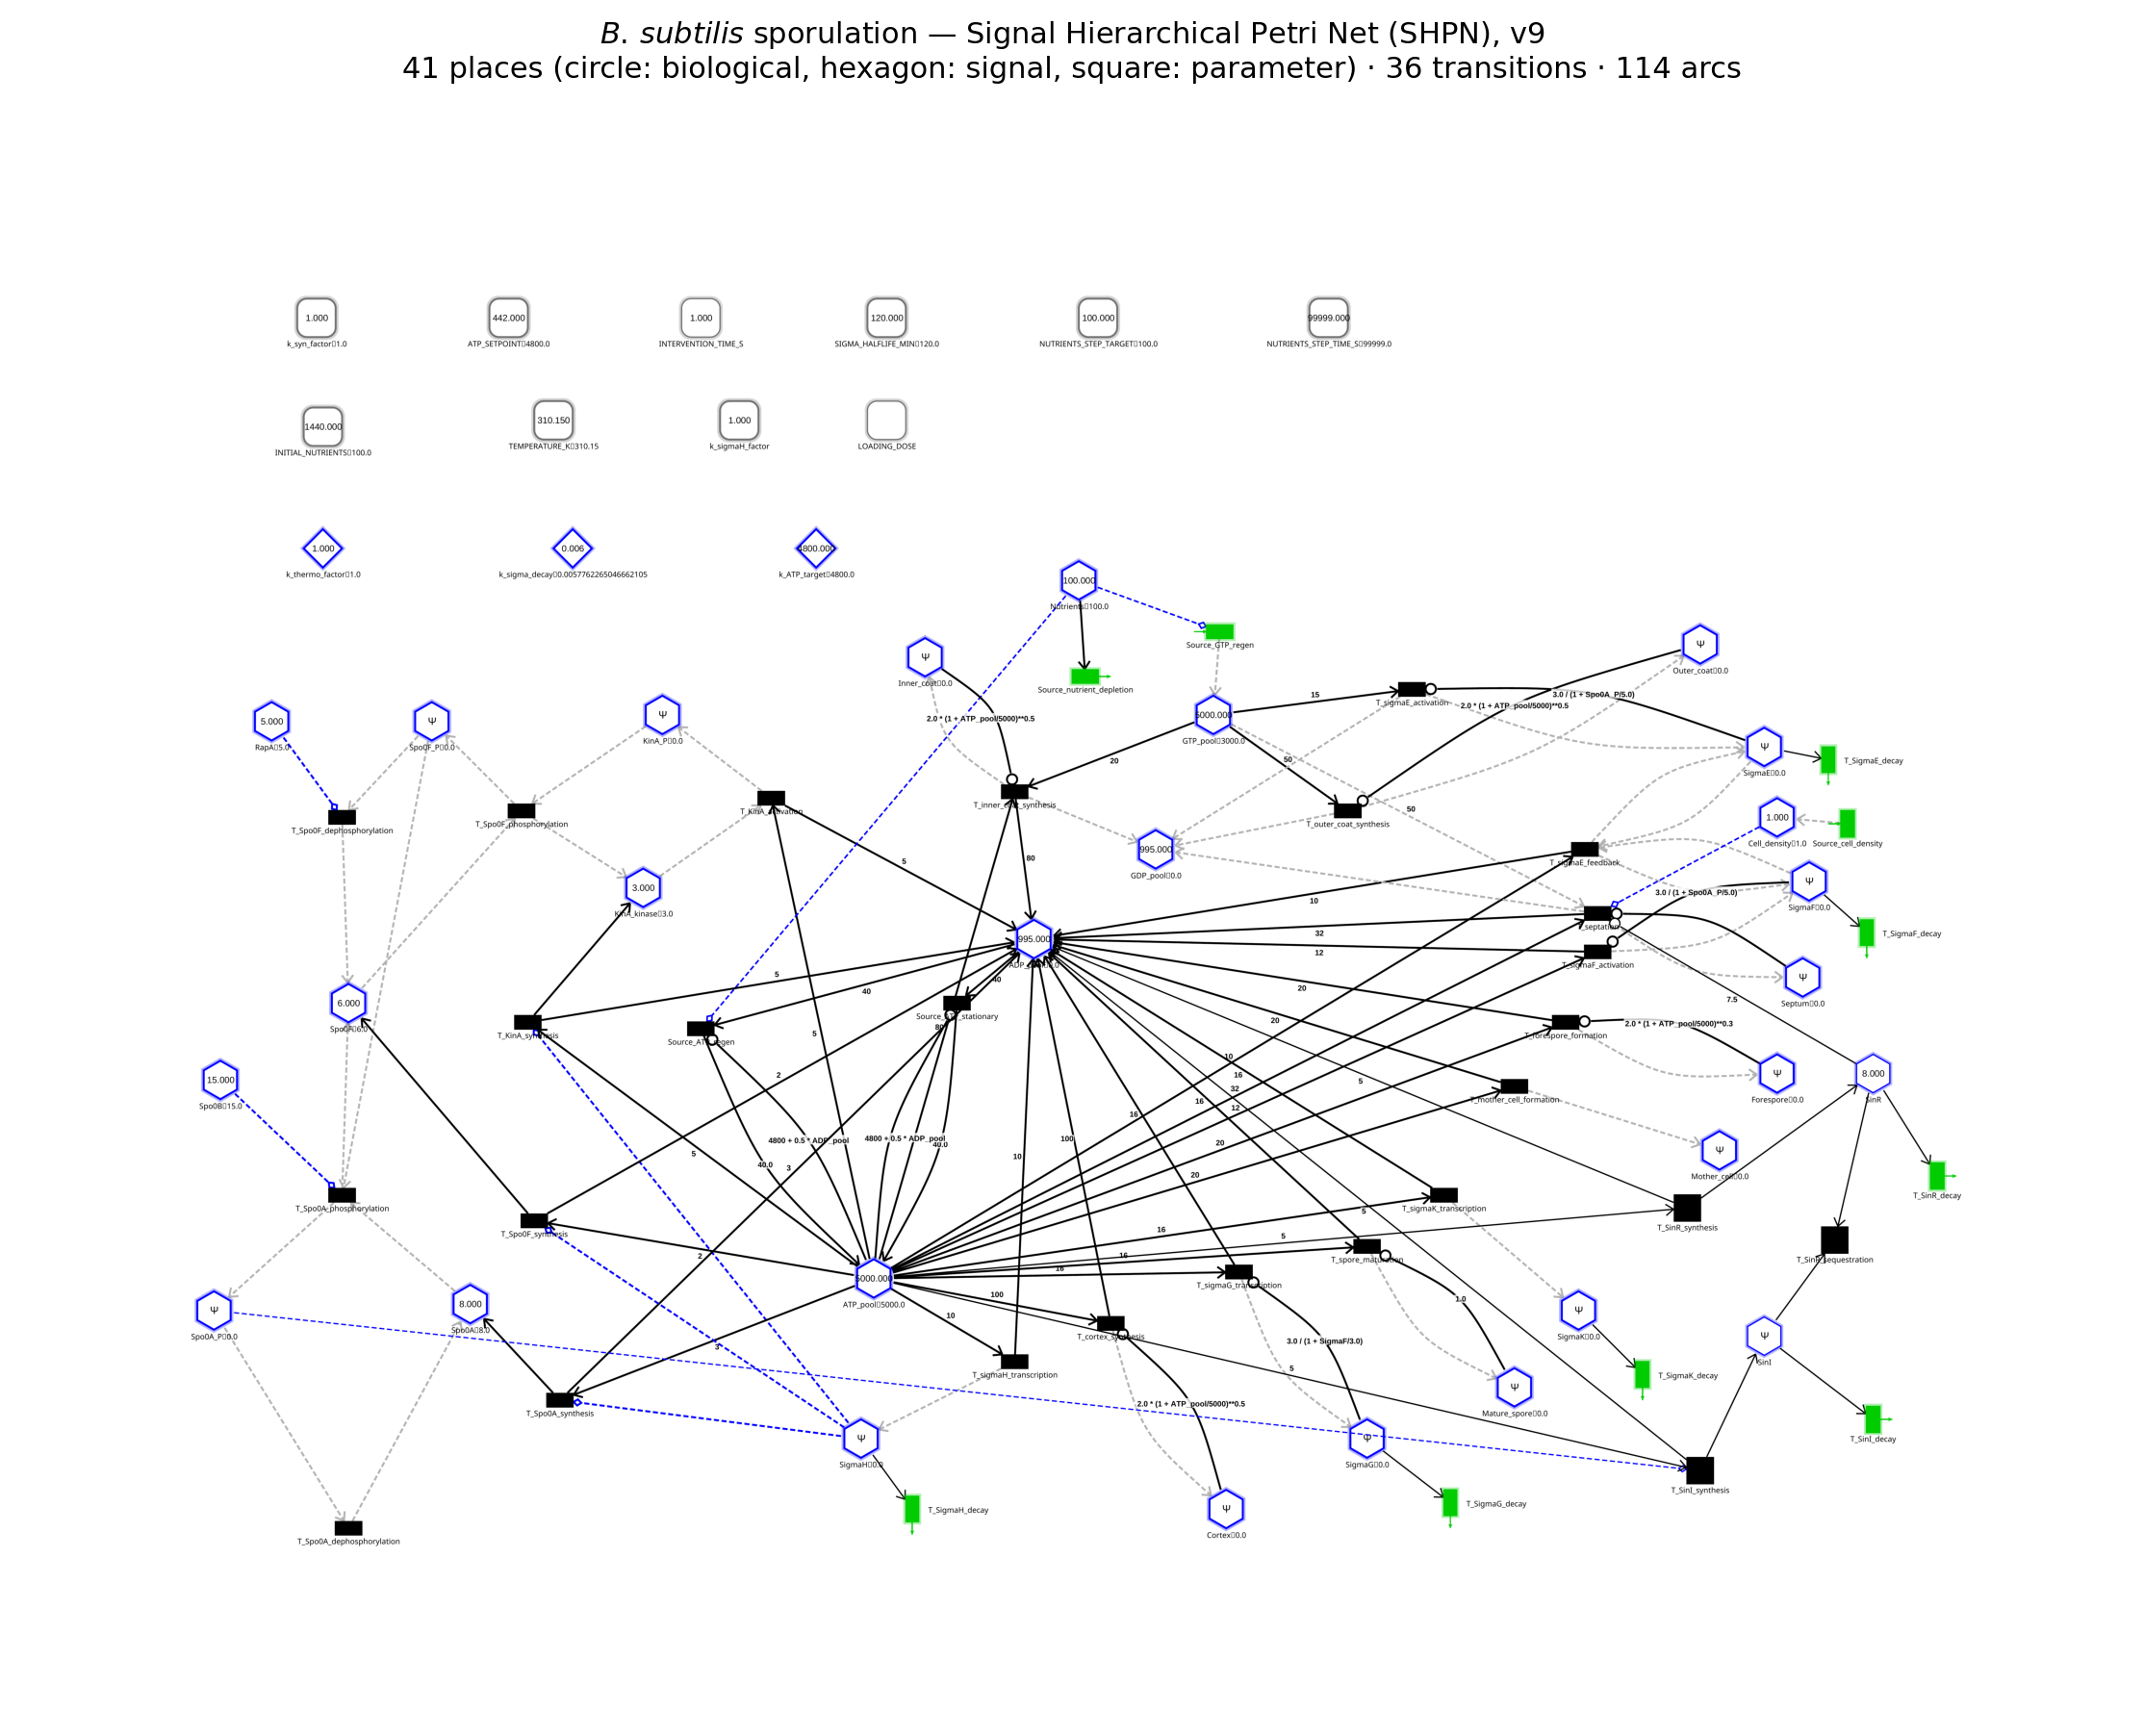
\includegraphics[width=0.9\linewidth]{figures/fig1_model.png}
  \caption{\textbf{SHPN v9 model of \textit{B.~subtilis} sporulation.}
  Circles: biological places ($\mu$M).
  Rectangles: transitions (stochastic = dashed border; ODE = solid).
  Hexagons: signal places ($\Psi$).
  Arc styles: solid black = normal; dashed blue = test;
  dashed grey = signal-flow; filled-circle head = inhibitor.
  Layer~A (commitment, stochastic, upper-left cluster) and Layer~B
  (execution, ODE, right) are structurally separated in the arc graph.}
  \label{fig:model}
\end{figure}

\subsection{Simulation protocol}

All simulations used the SHPN $\tau$-leaping engine
($\Delta t = 0.01$\,s, $\tau_{\mathrm{max}} = 0.01$\,s to suppress
Poisson over-sampling of low-copy transitions).
Each condition used $n = 50$ stochastic replicates over a 6-hour
horizon.
Sporulation was scored when at least one Mature\_spore token was
present at $t = 6$\,h.
EPR was computed per-replicate from firing counts using
\cref{eq:traj_epr}.

For the critical exponent analysis (\Cref{sec:results_thermo}), a
dense nutrient grid (1200--1550\,$\mu$M, 13 conditions) was used with
$n = 50$ replicates per condition.
$\CV^2_{\mathrm{bin}}$ was computed as $p(1-p)/p^2$ where $p$ is the
sporulation fraction; the fit used only sub-critical conditions
($N_0 < \Nc$) to avoid Bernoulli-dominated variance on the sup-critical
side.

\subsection{EPR computation}
\label{sec:methods_epr}

For each stochastic replicate trajectory $\omega$, the per-transition
EPR contribution at time $t$ is
\begin{equation}
  \EPR_t(\omega) = \frac{1}{\Delta t} \sum_{\rho \in t}
    k_\rho(\omega,t) \ln \frac{\Phi_\rho^+(M)}{\Phi_\rho^-(M)}
  \label{eq:epr_compute}
\end{equation}
where $k_\rho$ is the observed number of firings of elementary reaction
$\rho$ (forward or reverse) in $[t, t+\Delta t]$ and
$\Phi_\rho^\pm(M)$ are the propensities evaluated at the current marking.
This is the discrete-time approximation to \cref{eq:traj_epr}; the
error is $O(\Delta t)$.

Reversible reactions use the Skellam sampler
($k_{\mathrm{net}} \sim \mathrm{Skellam}(\Phi^+\Delta t, \Phi^-\Delta t)$)
and the log-ratio is evaluated at the net firing direction.
ODE-regime transitions contribute $\EPR_t = J_t \ln(J_t^+/J_t^-)
\cdot \Delta t$ where $J_t^\pm$ are the continuous fluxes.

% ─────────────────────────────────────────────────────────────────────────────
\section{Results I: Biological Validation}
\label{sec:results_bio}
% ─────────────────────────────────────────────────────────────────────────────

% Note: this section is the prerequisite for thermodynamic analysis.
% The subnetwork model must be biologically grounded before NESM quantities
% can be trusted. Three experimental constraints from Fujita & Losick (2005)
% are reproduced.

Before thermodynamic analysis, the SHPN model must be validated against
established experimental constraints.
Fujita \& Losick~\cite{Fujita2005} characterised three properties of
\textit{B.~subtilis} sporulation commitment that any model must
reproduce.
We address them in order.

\subsection{Q1: Commitment route and metabolic state (Fujita Fig.\ 3)}

[CONTENT: port from plos_one_how_cells_decide.tex Results section for FUJITA-1.
Include Fig 2 (fig2_q1_gate.png) and the sporulation \% table.
Brief: 1 page max.]

\subsection{Q2: $\sigma_H$ is the irreversible gate (Fujita Fig.\ 4)}

[CONTENT: port from plos_one_how_cells_decide.tex Results section for FUJITA-3.
Include Fig 3 (fig3_q2_sigmaH.png).
Brief: 0.5 page max.]

\subsection{Q3: Nutrient threshold and commitment timing (Fujita Fig.\ 5)}

[CONTENT: port from plos_one_how_cells_decide.tex Results section for FUJITA-2/4.
Include Fig 4 (fig4_q3_Nc.png).
Brief: 0.5 page max.]

% ─────────────────────────────────────────────────────────────────────────────
\section{Results II: Thermodynamic Characterisation of Commitment}
\label{sec:results_thermo}
% ─────────────────────────────────────────────────────────────────────────────

\subsection{Topological load $\etaL$ and commitment modes (NET-T1)}
\label{sec:results_eta}

[CONTENT: NET-T1 analysis — eta_L topology-constancy, two commitment modes.
Include Fig 5 left panel (from fig5_thermo_cost.png).
~0.75 page.]

\subsection{Free energy landscape and dissipative work (NET-T2, NET-T3)}
\label{sec:results_landscape}

[CONTENT: Waddington landscape, W/kBT = 3.72e7, FT inapplicability,
FWD/REV perturbation asymmetry.
Include Fig 5 right panel + Fig 6a (fig6a_waddington.png).
~1 page.]

\subsection{Non-mean-field critical transition near $\Nc$ (NET-T4)}
\label{sec:results_critical}

The sub-critical scaling of $\CV^2_{\mathrm{bin}}$ follows
\cref{eq:gsub} with fitted exponent $\gsub = 0.150 \pm 0.044$
($R^2 = 0.694$, $n = 7$ sub-critical conditions, $p < 10^{-6}$).
This is $19\sigma$ below the mean-field prediction $\gsub^{\mathrm{MF}} = 0.5$.

The critical threshold is $\Nc = 1346\,\mu$M, identified as the
nutrient level at which sporulation probability crosses 50\%.
Critical slowing-down is observed: the mean commitment time rises from
317\,min at $N_0 = 1250\,\mu$M to 337\,min at $N_0 = 1345\,\mu$M,
a 6.3\% increase over 95\,$\mu$M --- the characteristic divergence of the
relaxation time near a second-order transition.

Near $\Nc$, the $\sigma_H$ peak concentration remains below the
activation threshold $\theta_{\sigma H} = 1.60\,\mu$M, so the commitment
probability is $P(\mathrm{spor}) = P(\sigma_H > \theta_{\sigma H})$ ---
a threshold-crossing probability driven by stochastic fluctuations in
Layer~A, not a deterministic crossing.

[CONTENT: Include Fig 6b (fig6b_critical_exponents.png) with the log-log
CV^2 vs |N0-Nc| fit.]

\subsection{Entropy production decomposition (NET-T5)}
\label{sec:results_epr}

[CONTENT: EPR decomposition — KinA 97.5%, septation asymmetry 14.3x,
total EPR 5.6->0.9->~0 kBT/s.
Include Fig 7 (fig7_epr.png).
~1 page.]

% ─────────────────────────────────────────────────────────────────────────────
\section{Discussion}
\label{sec:discussion}
% ─────────────────────────────────────────────────────────────────────────────

\subsection{The physical origin of the non-mean-field universality class}

[CONTENT: Why gamma != 0.5. Phosphorelay cascade + SinR gate introduces
effective long-range correlations. PreemptionCheck couples Layer A
transitions. Connection to non-MF universality in statistical physics.
~0.5 page.]

\subsection{The Markovian reservoir assumption: scope and limitations}

[CONTENT: When does it hold? When does it break?
Deep starvation / starved-refed experiments.
Empirical verification via Fujita.
Honest scope statement.
~0.4 page.]

\subsection{Topology encodes thermodynamics}

[CONTENT: eta_L topology-constancy (NET-T1).
EPR bottleneck at KinA is structural.
Connection to Thermodynamic Uncertainty Relations (TUR, Barato & Seifert 2015).
The bet-hedging window is the regime of deliberately low precision / high
population diversity.
~0.5 page.]

\subsection{Generality of the framework}

[CONTENT: The five quantities are computable for any SHPN with known topology.
Candidate circuits: Caulobacter CtrA/DnaA, E. coli SOS (LexA/RecA),
mammalian apoptosis (Bcl-2 family).
No new experiments required — extract thermodynamics from existing validated models.
~0.3 page.]

% ─────────────────────────────────────────────────────────────────────────────
\section{Conclusion}
\label{sec:conclusion}
% ─────────────────────────────────────────────────────────────────────────────

We have shown that single-cell commitment decisions have a computable
thermodynamic characterisation within the NESM framework when modelled
with the SHPN formalism.
The arc semantics of the SHPN map directly onto the thermodynamic ports
of an open driven Markov system, and five quantities derivable from
topology and stochastic dynamics alone constitute a thermodynamic
fingerprint of the commitment circuit.

For \textit{B.~subtilis} sporulation, this fingerprint reveals:
the commitment transition is non-mean-field ($\gsub = 0.150 \pm 0.044$);
the critical nutrient threshold is $\Nc = 1346\,\mu$M;
the thermodynamic cost of commitment is overwhelmingly concentrated at
the sensing step, not the execution programme;
and the bet-hedging population window (700--1800\,$\mu$M) corresponds
to the regime where the Thermodynamic Uncertainty Relation allows
maximum population diversity at the cost of single-cell decision precision.

The Markovian reservoir assumption restricts the quantitative claims to
the decision window under starvation conditions.
Extending the framework to include metabolic dynamics and full-lifecycle
thermodynamics is a direct next step.
More broadly, the SHPN provides a ready substrate for computing the
thermodynamic fingerprint of any regulatory commitment circuit whose
topology and stochastic rates are known --- a new measurement handle on
the physics of cellular decision-making.

% ─────────────────────────────────────────────────────────────────────────────
%  REFERENCES  (placeholder — replace with BibTeX)
% ─────────────────────────────────────────────────────────────────────────────
\begin{thebibliography}{99}

\bibitem{Seifert2012}
  Seifert, U. (2012).
  Stochastic thermodynamics, fluctuation theorems and molecular machines.
  \textit{Reports on Progress in Physics}, \textbf{75}(12), 126001.

\bibitem{Seifert2005}
  Seifert, U. (2005).
  Entropy production along a stochastic trajectory and an integral
  fluctuation theorem.
  \textit{Physical Review Letters}, \textbf{95}, 040602.

\bibitem{Rao2018}
  Rao, R.\ \& Esposito, M. (2018).
  Conservation laws and work fluctuation relations in chemical reaction networks.
  \textit{New Journal of Physics}, \textbf{20}, 023007.

\bibitem{Esposito2010}
  Esposito, M.\ \& Van den Broeck, C. (2010).
  Three faces of the second law. I. Master equation formulation.
  \textit{Physical Review Letters}, \textbf{104}, 090601.

\bibitem{Barato2015}
  Barato, A.C.\ \& Seifert, U. (2015).
  Thermodynamic uncertainty relation for biomolecular processes.
  \textit{Physical Review Letters}, \textbf{114}, 158101.

\bibitem{Schnakenberg1976}
  Schnakenberg, J. (1976).
  Network theory of microscopic and macroscopic behavior of master equation
  systems.
  \textit{Reviews of Modern Physics}, \textbf{48}, 571.

\bibitem{Jarzynski1997}
  Jarzynski, C. (1997).
  Nonequilibrium equality for free energy differences.
  \textit{Physical Review Letters}, \textbf{78}, 2690.

\bibitem{Crooks1999}
  Crooks, G.E. (1999).
  Entropy production fluctuation theorem and the nonequilibrium work
  relation for free energy differences.
  \textit{Physical Review E}, \textbf{60}, 2721.

\bibitem{Liphardt2002}
  Liphardt, J., Dumont, S., Smith, S.B., Tinoco, I.\ \& Bustamante, C. (2002).
  Equilibrium information from nonequilibrium measurements in an experimental
  test of Jarzynski's equality.
  \textit{Science}, \textbf{296}, 1832--1835.

\bibitem{Wang2002}
  Wang, G.M., Sevick, E.M., Mittag, E., Searles, D.J.\ \& Evans, D.J. (2002).
  Experimental demonstration of violations of the second law of thermodynamics
  for small systems and short time scales.
  \textit{Physical Review Letters}, \textbf{89}, 050601.

\bibitem{Gillespie2001}
  Gillespie, D.T. (2001).
  Approximate accelerated stochastic simulation of chemically reacting systems.
  \textit{Journal of Chemical Physics}, \textbf{115}, 1716.

\bibitem{Hill1977}
  Hill, T.L. (1977).
  \textit{Free Energy Transduction in Biology.} Academic Press, New York.

\bibitem{Fujita2005}
  Fujita, M.\ \& Losick, R. (2005).
  Evidence that entry into sporulation in \textit{Bacillus subtilis} is
  governed by a gradual increase in the level and activity of the master
  regulator Spo0A.
  \textit{Genes \& Development}, \textbf{19}, 2236--2244.

\bibitem{Losick2008}
  Losick, R.\ \& Desplan, C. (2008).
  Stochasticity and cell fate.
  \textit{Science}, \textbf{320}, 65--68.

\bibitem{Simao2025}
  Sim\~{a}o, E. (2025).
  Signal Hierarchical Petri Nets for biological systems: formalism,
  engine, and thermodynamic extensions.
  [Preprint / manuscript in preparation]

\end{thebibliography}

\end{document}
